% Options for packages loaded elsewhere
\PassOptionsToPackage{unicode}{hyperref}
\PassOptionsToPackage{hyphens}{url}
\PassOptionsToPackage{dvipsnames,svgnames,x11names}{xcolor}
%
\documentclass[
]{article}
\usepackage{amsmath,amssymb}
\usepackage{lmodern}
\usepackage{iftex}
\ifPDFTeX
  \usepackage[T1]{fontenc}
  \usepackage[utf8]{inputenc}
  \usepackage{textcomp} % provide euro and other symbols
\else % if luatex or xetex
  \usepackage{unicode-math}
  \defaultfontfeatures{Scale=MatchLowercase}
  \defaultfontfeatures[\rmfamily]{Ligatures=TeX,Scale=1}
\fi
% Use upquote if available, for straight quotes in verbatim environments
\IfFileExists{upquote.sty}{\usepackage{upquote}}{}
\IfFileExists{microtype.sty}{% use microtype if available
  \usepackage[]{microtype}
  \UseMicrotypeSet[protrusion]{basicmath} % disable protrusion for tt fonts
}{}
\makeatletter
\@ifundefined{KOMAClassName}{% if non-KOMA class
  \IfFileExists{parskip.sty}{%
    \usepackage{parskip}
  }{% else
    \setlength{\parindent}{0pt}
    \setlength{\parskip}{6pt plus 2pt minus 1pt}}
}{% if KOMA class
  \KOMAoptions{parskip=half}}
\makeatother
\usepackage{xcolor}
\usepackage[margin=1in]{geometry}
\usepackage{color}
\usepackage{fancyvrb}
\newcommand{\VerbBar}{|}
\newcommand{\VERB}{\Verb[commandchars=\\\{\}]}
\DefineVerbatimEnvironment{Highlighting}{Verbatim}{commandchars=\\\{\}}
% Add ',fontsize=\small' for more characters per line
\usepackage{framed}
\definecolor{shadecolor}{RGB}{248,248,248}
\newenvironment{Shaded}{\begin{snugshade}}{\end{snugshade}}
\newcommand{\AlertTok}[1]{\textcolor[rgb]{0.94,0.16,0.16}{#1}}
\newcommand{\AnnotationTok}[1]{\textcolor[rgb]{0.56,0.35,0.01}{\textbf{\textit{#1}}}}
\newcommand{\AttributeTok}[1]{\textcolor[rgb]{0.77,0.63,0.00}{#1}}
\newcommand{\BaseNTok}[1]{\textcolor[rgb]{0.00,0.00,0.81}{#1}}
\newcommand{\BuiltInTok}[1]{#1}
\newcommand{\CharTok}[1]{\textcolor[rgb]{0.31,0.60,0.02}{#1}}
\newcommand{\CommentTok}[1]{\textcolor[rgb]{0.56,0.35,0.01}{\textit{#1}}}
\newcommand{\CommentVarTok}[1]{\textcolor[rgb]{0.56,0.35,0.01}{\textbf{\textit{#1}}}}
\newcommand{\ConstantTok}[1]{\textcolor[rgb]{0.00,0.00,0.00}{#1}}
\newcommand{\ControlFlowTok}[1]{\textcolor[rgb]{0.13,0.29,0.53}{\textbf{#1}}}
\newcommand{\DataTypeTok}[1]{\textcolor[rgb]{0.13,0.29,0.53}{#1}}
\newcommand{\DecValTok}[1]{\textcolor[rgb]{0.00,0.00,0.81}{#1}}
\newcommand{\DocumentationTok}[1]{\textcolor[rgb]{0.56,0.35,0.01}{\textbf{\textit{#1}}}}
\newcommand{\ErrorTok}[1]{\textcolor[rgb]{0.64,0.00,0.00}{\textbf{#1}}}
\newcommand{\ExtensionTok}[1]{#1}
\newcommand{\FloatTok}[1]{\textcolor[rgb]{0.00,0.00,0.81}{#1}}
\newcommand{\FunctionTok}[1]{\textcolor[rgb]{0.00,0.00,0.00}{#1}}
\newcommand{\ImportTok}[1]{#1}
\newcommand{\InformationTok}[1]{\textcolor[rgb]{0.56,0.35,0.01}{\textbf{\textit{#1}}}}
\newcommand{\KeywordTok}[1]{\textcolor[rgb]{0.13,0.29,0.53}{\textbf{#1}}}
\newcommand{\NormalTok}[1]{#1}
\newcommand{\OperatorTok}[1]{\textcolor[rgb]{0.81,0.36,0.00}{\textbf{#1}}}
\newcommand{\OtherTok}[1]{\textcolor[rgb]{0.56,0.35,0.01}{#1}}
\newcommand{\PreprocessorTok}[1]{\textcolor[rgb]{0.56,0.35,0.01}{\textit{#1}}}
\newcommand{\RegionMarkerTok}[1]{#1}
\newcommand{\SpecialCharTok}[1]{\textcolor[rgb]{0.00,0.00,0.00}{#1}}
\newcommand{\SpecialStringTok}[1]{\textcolor[rgb]{0.31,0.60,0.02}{#1}}
\newcommand{\StringTok}[1]{\textcolor[rgb]{0.31,0.60,0.02}{#1}}
\newcommand{\VariableTok}[1]{\textcolor[rgb]{0.00,0.00,0.00}{#1}}
\newcommand{\VerbatimStringTok}[1]{\textcolor[rgb]{0.31,0.60,0.02}{#1}}
\newcommand{\WarningTok}[1]{\textcolor[rgb]{0.56,0.35,0.01}{\textbf{\textit{#1}}}}
\usepackage{graphicx}
\makeatletter
\def\maxwidth{\ifdim\Gin@nat@width>\linewidth\linewidth\else\Gin@nat@width\fi}
\def\maxheight{\ifdim\Gin@nat@height>\textheight\textheight\else\Gin@nat@height\fi}
\makeatother
% Scale images if necessary, so that they will not overflow the page
% margins by default, and it is still possible to overwrite the defaults
% using explicit options in \includegraphics[width, height, ...]{}
\setkeys{Gin}{width=\maxwidth,height=\maxheight,keepaspectratio}
% Set default figure placement to htbp
\makeatletter
\def\fps@figure{htbp}
\makeatother
\setlength{\emergencystretch}{3em} % prevent overfull lines
\providecommand{\tightlist}{%
  \setlength{\itemsep}{0pt}\setlength{\parskip}{0pt}}
\setcounter{secnumdepth}{-\maxdimen} % remove section numbering
\usepackage{amsmath}
\ifLuaTeX
  \usepackage{selnolig}  % disable illegal ligatures
\fi
\IfFileExists{bookmark.sty}{\usepackage{bookmark}}{\usepackage{hyperref}}
\IfFileExists{xurl.sty}{\usepackage{xurl}}{} % add URL line breaks if available
\urlstyle{same} % disable monospaced font for URLs
\hypersetup{
  pdftitle={Compulsory Exercise 2: Title (give your project an informative title)},
  pdfauthor={Full name for group member \#1.; Full name for group member \#2.; Full name for group member \#3.},
  colorlinks=true,
  linkcolor={Maroon},
  filecolor={Maroon},
  citecolor={Blue},
  urlcolor={blue},
  pdfcreator={LaTeX via pandoc}}

\title{Compulsory Exercise 2: Title (give your project an informative
title)}
\author{Full name for group member \#1. \and Full name for group member
\#2. \and Full name for group member \#3.}
\date{15 april, 2023}

\begin{document}
\maketitle
\begin{abstract}
This is the place for your abstract (max 350 words)
\end{abstract}

\hypertarget{introduction-scope-and-purpose-of-your-project}{%
\subsection{Introduction: Scope and purpose of your
project}\label{introduction-scope-and-purpose-of-your-project}}

\hypertarget{descriptive-data-analysisstatistics}{%
\subsection{Descriptive data
analysis/statistics}\label{descriptive-data-analysisstatistics}}

We load in the data set, and change the data type of all categorical
variables to factor variables so that r knows the right encoding.

\begin{Shaded}
\begin{Highlighting}[]
\NormalTok{heart }\OtherTok{\textless{}{-}} \FunctionTok{read.csv}\NormalTok{(}\StringTok{"heart.csv"}\NormalTok{)}
\NormalTok{heart}\SpecialCharTok{$}\NormalTok{Sex }\OtherTok{\textless{}{-}} \FunctionTok{factor}\NormalTok{(heart}\SpecialCharTok{$}\NormalTok{Sex)}
\NormalTok{heart}\SpecialCharTok{$}\NormalTok{ChestPainType }\OtherTok{\textless{}{-}} \FunctionTok{factor}\NormalTok{(heart}\SpecialCharTok{$}\NormalTok{ChestPainType)}
\NormalTok{heart}\SpecialCharTok{$}\NormalTok{FastingBS }\OtherTok{\textless{}{-}} \FunctionTok{factor}\NormalTok{(heart}\SpecialCharTok{$}\NormalTok{FastingBS)}
\NormalTok{heart}\SpecialCharTok{$}\NormalTok{RestingECG }\OtherTok{\textless{}{-}} \FunctionTok{factor}\NormalTok{(heart}\SpecialCharTok{$}\NormalTok{RestingECG)}
\NormalTok{heart}\SpecialCharTok{$}\NormalTok{ExerciseAngina }\OtherTok{\textless{}{-}} \FunctionTok{factor}\NormalTok{(heart}\SpecialCharTok{$}\NormalTok{ExerciseAngina)}
\NormalTok{heart}\SpecialCharTok{$}\NormalTok{ST\_Slope }\OtherTok{\textless{}{-}} \FunctionTok{factor}\NormalTok{(heart}\SpecialCharTok{$}\NormalTok{ST\_Slope)}
\NormalTok{heart}\SpecialCharTok{$}\NormalTok{HeartDisease }\OtherTok{\textless{}{-}} \FunctionTok{factor}\NormalTok{(heart}\SpecialCharTok{$}\NormalTok{HeartDisease)}
\end{Highlighting}
\end{Shaded}

Then we run the \textbf{dim} and \textbf{summary} functions to get a
quick overview of the data.

\begin{Shaded}
\begin{Highlighting}[]
\FunctionTok{dim}\NormalTok{ (heart)}
\end{Highlighting}
\end{Shaded}

\begin{verbatim}
## [1] 918  12
\end{verbatim}

\begin{Shaded}
\begin{Highlighting}[]
\FunctionTok{summary}\NormalTok{(heart)}
\end{Highlighting}
\end{Shaded}

\begin{verbatim}
##       Age        Sex     ChestPainType   RestingBP      Cholesterol   
##  Min.   :28.00   F:193   ASY:496       Min.   :  0.0   Min.   :  0.0  
##  1st Qu.:47.00   M:725   ATA:173       1st Qu.:120.0   1st Qu.:173.2  
##  Median :54.00           NAP:203       Median :130.0   Median :223.0  
##  Mean   :53.51           TA : 46       Mean   :132.4   Mean   :198.8  
##  3rd Qu.:60.00                         3rd Qu.:140.0   3rd Qu.:267.0  
##  Max.   :77.00                         Max.   :200.0   Max.   :603.0  
##  FastingBS  RestingECG      MaxHR       ExerciseAngina    Oldpeak       
##  0:704     LVH   :188   Min.   : 60.0   N:547          Min.   :-2.6000  
##  1:214     Normal:552   1st Qu.:120.0   Y:371          1st Qu.: 0.0000  
##            ST    :178   Median :138.0                  Median : 0.6000  
##                         Mean   :136.8                  Mean   : 0.8874  
##                         3rd Qu.:156.0                  3rd Qu.: 1.5000  
##                         Max.   :202.0                  Max.   : 6.2000  
##  ST_Slope   HeartDisease
##  Down: 63   0:410       
##  Flat:460   1:508       
##  Up  :395               
##                         
##                         
## 
\end{verbatim}

We find that the data set contains 918 rows and and 12 columns. The
twelve columns are: \textbf{Age, Sex, ChestPainType, RestingBP,
Cholesterol, FastingBS, RestingECG, MaxHR, ExerciseAngina, Oldpeak,
ST\_Slope} and \textbf{HeartDisease}. \#\#Tror dette egentlig burde i
introduction delen\#\#. From the output of \textbf{summary} one can see
the min, max, mean and median for all numerical variables and the
distribution of the categorical variables. We notice that the data set
contains significantly fewer women than men, which might skew the effect
of \textbf{Sex} on the target variable. The same goes for \textbf{Age}
as over half the people are between 45 and 60 years, which is about 25
\% of the total age range of 28 to 77.

To get a better view of the data we use the \textbf{ggpairs} function.

\begin{Shaded}
\begin{Highlighting}[]
\FunctionTok{ggpairs}\NormalTok{(heart)}
\end{Highlighting}
\end{Shaded}

\begin{figure}

{\centering 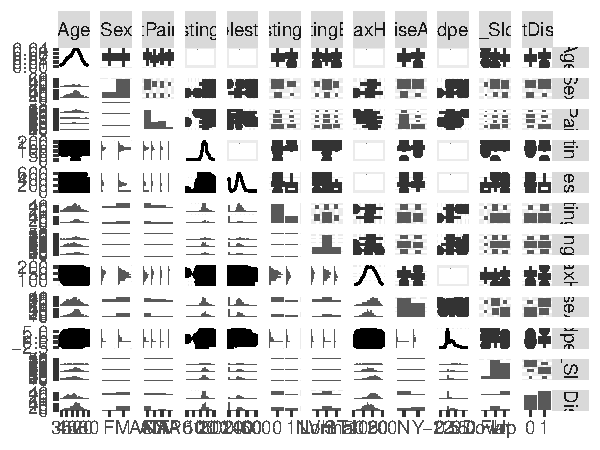
\includegraphics{Main_Text_files/figure-latex/unnamed-chunk-4-1} 

}

\caption{pairplot}\label{fig:unnamed-chunk-4}
\end{figure}

From \textbf{figure XXX} we can se the distribution of all the
variables, and we can see them plotted against each other. We also see
the correlation between the numerical covariates, and notice that none
of them seem to be highly correlated. \textbf{MaxHR} and \textbf{Age}
have the largest value of - 0.382 which is indicates a moderate negative
correlation between the two variables.

\hypertarget{methods}{%
\subsection{Methods}\label{methods}}

\hypertarget{results-and-interpretation}{%
\subsection{Results and
interpretation}\label{results-and-interpretation}}

\hypertarget{summary}{%
\subsection{Summary}\label{summary}}

\end{document}
